%************************************************
\chapter{Image Preprocessing}\label{ch:mathtest} % $\mathbb{ZNR}$
%************************************************
To perform most automated analyses on neuroimaging, it is fundamental that images are comparable. Preprocessing comprises a series of algorithms that, applied after the acquisition and reconstruction of the images, produce directly comparable images in both structure and magnitude. 

In this section we present the preprocessing algorithms used in this thesis. Whether they have been used in one or all experiments, they can be classified in two major categories: spatial and intensity preprocessing. Later, in Section~\ref{sec:vwanalyses}, we present some voxelwise analyses, commonly used in clinical practice, that we have set as a baseline in our experiments. 

\section{Spatial Preprocessing }
Spatial processing usually accounts for the differences in position, angles and structure that are commonly found between images. A common pipeline in, for example, \ac{MRI} preprocessing, is the one found at Figure~\ref{fig:examplePreMRI}, where the images are registered (or spatially normalized) to a template, smoothed and finally segmented. The smoothing is an optional step, generally used in procedures like segmentation or \ac{VBM}. 

\begin{figure}[htp]
	\myfloatalign
	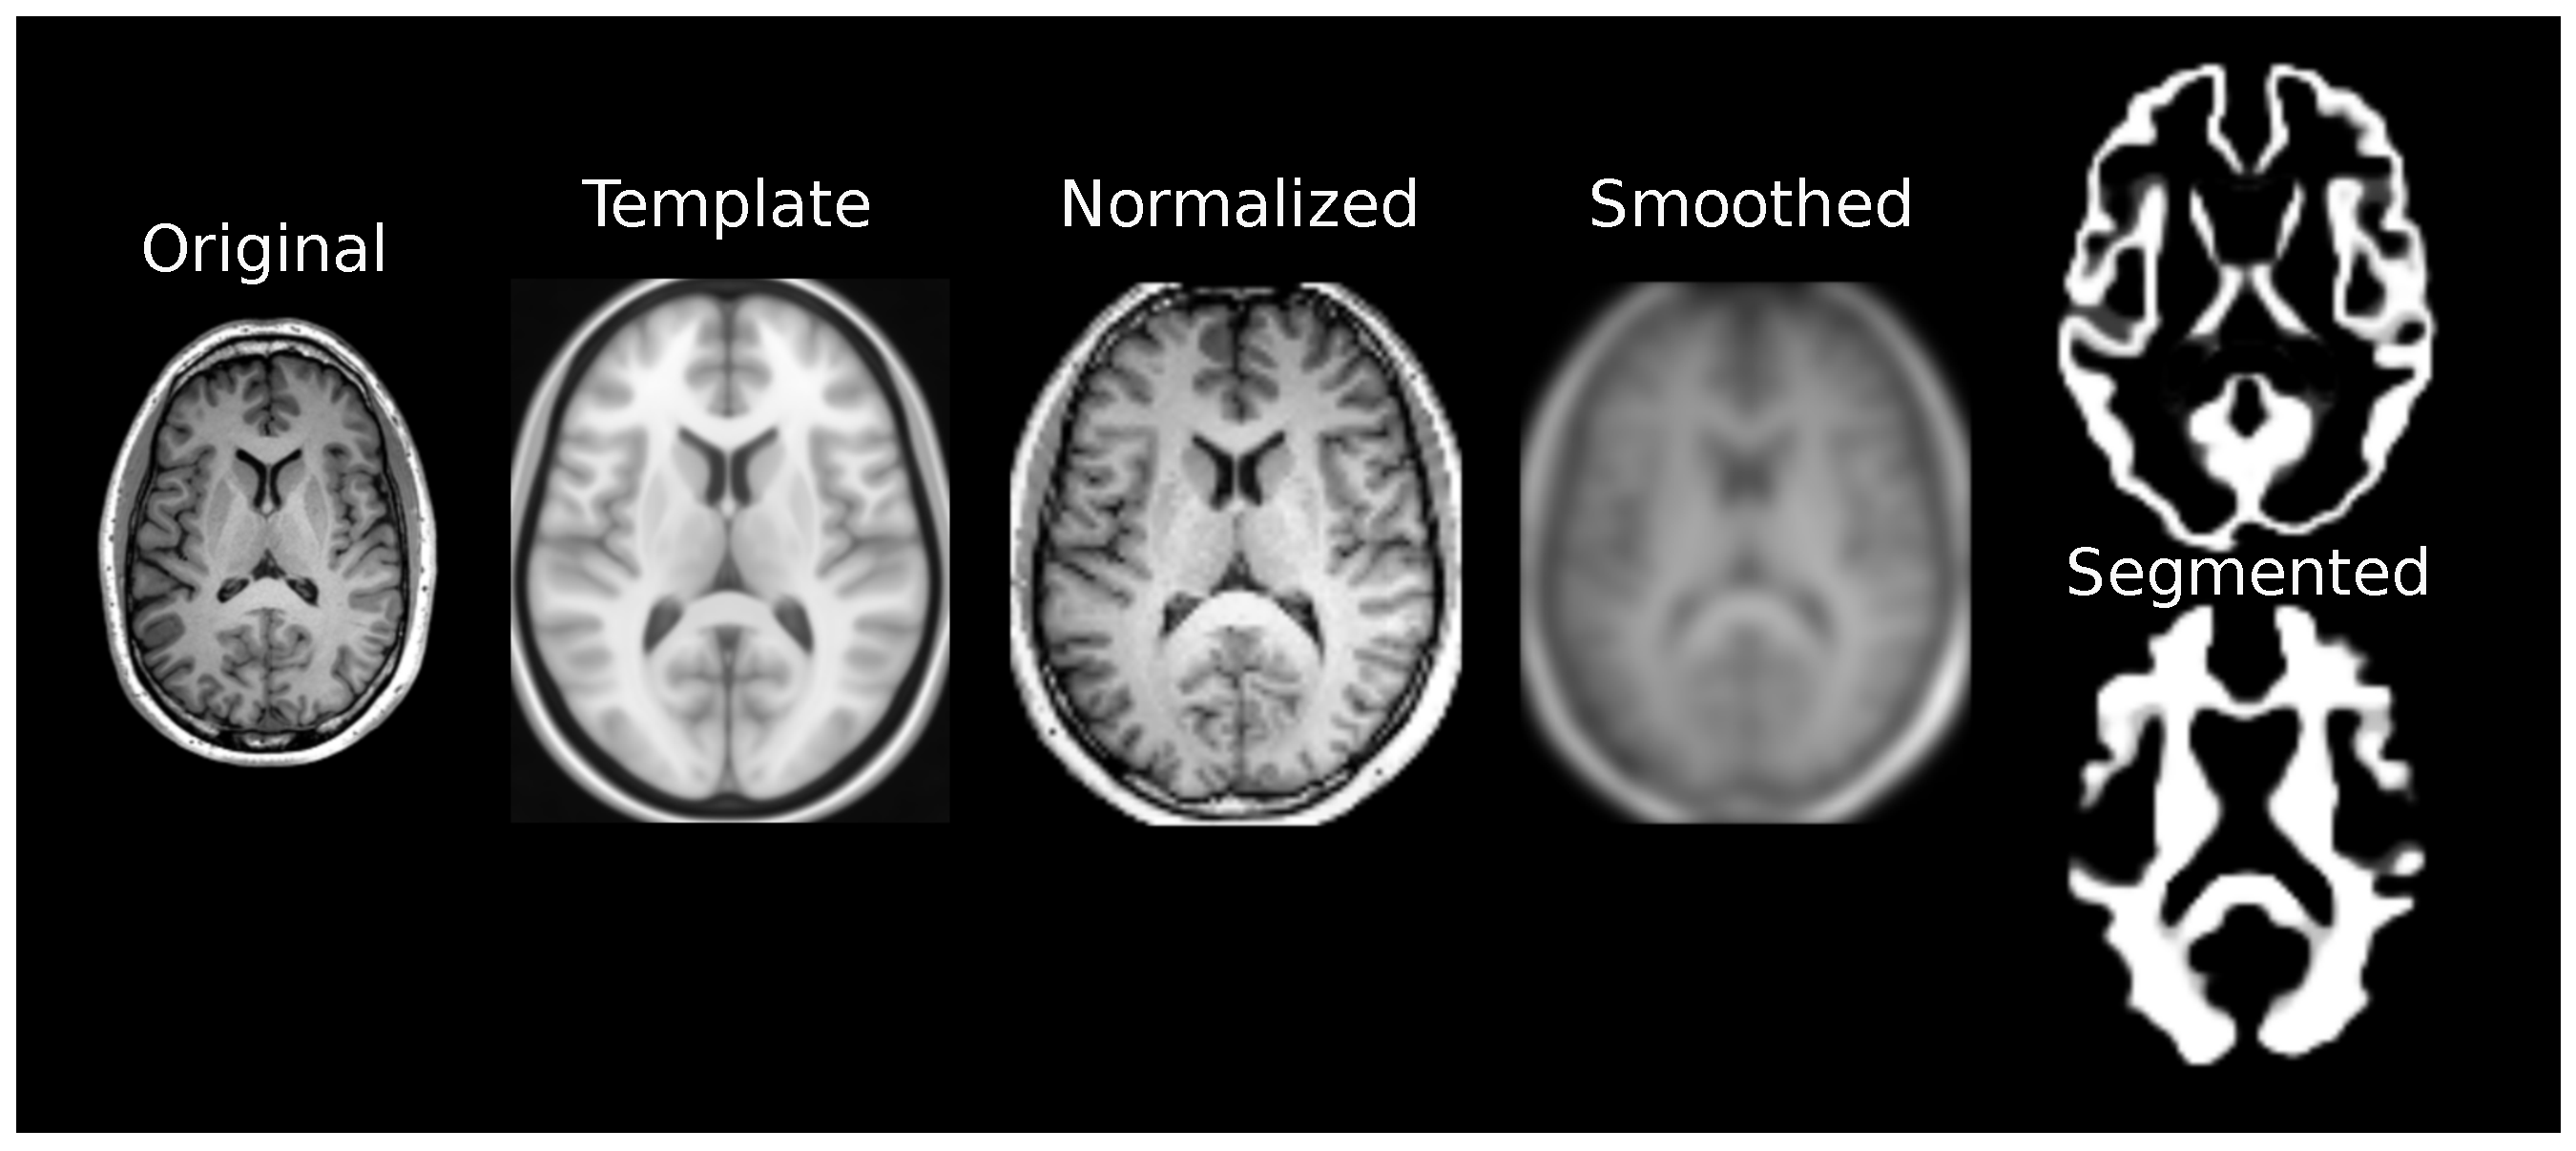
\includegraphics[width=.75\linewidth]{gfx/ch3/preProcessPL}
	\caption[Typical pre-processing pipeline in MRI]{Typical pre-processing pipeline in \ac{MRI}.}\label{fig:examplePreMRI}
\end{figure}

In this thesis, all the experiments in all image modalities involve spatial normalization. Smoothing, as well as segmentation, is only applied in some experiments that use \ac{MRI} images, such as the segmented images in Chapter~\ref{ch:sbm} or the whole-brain analysis performed in Chapter~\ref{ch:swpca}. 

\subsection{Spatial Normalization or Registration}
Spatial Normalization, also known as Registration, is the procedure that by which every subject's brain is mapped from their individual space to a standard reference system. Registered images allows our system to overcome the individual differences in position and anatomy by establishing a common reference space in which a given coordinate represent the same anatomical position in all brains in the dataset. 

There exist a number of pieces of software widely used for registering images, such as FreeSurfer \cite{Reuter2010} or FSL (in the FLIRT and FNIRT package) \cite{Smith2004}, most of them perform linear, non-rigid and elastic transformations or a combination of these. In this work we have used the software SPM8 \cite{spm_book} to perform registration of all the datasets, including \ac{MRI}, \ac{SPECT} and \ac{PET} images. So, from this moment, we will focus on the registration as performed in the \ac{SPM8}. 

Linear registration usually refers to the affine transformation, a matrix multiplication that includes 12 parameters for translation, rotation, scale, squeeze, shear and others: 
\begin{equation}\label{eq:affine}
	\left[\begin{matrix}
	x'\\y'\\z'\\1
	\end{matrix}\right]
	 = \left[\begin{matrix}
	 a_{00} & a_{01} & a_{02} & a_{03}\\
	 a_{10} & a_{11} & a_{12} & a_{13}\\
	 a_{20} & a_{21} & a_{22} & a_{23}\\
	 0 & 0 & 0 & 1\\
	 \end{matrix}\right]
	 \left[\begin{matrix}
	 x\\y\\z\\1
	 \end{matrix}\right]
\end{equation}

This matrix multiplication is performed globally, as it transforms the whole image, not accounting for local geometric differences. In equations \ref{eq:affine1}, \ref{eq:affine2} and \ref{eq:affine3} we give an example of the parameters that are computed for scale, translation and shear in 3D:

\begin{align}
\label{eq:affine1}
	\text{scale} &= 
	\left[\begin{matrix}
		 s_x  &0 & 0 & 0\\
		0 &s_y &0 &0\\
		0 &0 &s_z &0\\
		0 &0 &0 &1		
	\end{matrix}
	\right]\\
	\label{eq:affine2}
	\text{translation} &= 
	\left[
	\begin{matrix}
	1  &0 & 0 & \Delta x\\
	0 &1 &0 &\Delta y\\
	0 &0 &1 &\Delta z\\
	0 &0 &0 &1		
	\end{matrix}
	\right] \\
	\label{eq:affine3}
	\text{shear} &= 
	\left[\begin{matrix}
	1  &h_{xy}& h_{xz} & 0\\
	h_{yx} &1 &h_{yz} &0\\
	h_{zx} &h_{zy} &1 &0\\
	0 &0 &0 &1		
	\end{matrix}
	\right]
\end{align}

The combination of all these operations result in the estimation of the twelve parameters that we found in Eq.~\ref{eq:affine}, which are the ones used in \ac{SPM8}. The estimation of these parameters is performed via the optimization of a cost function, that in \ac{SPM8} can be the minimum squared difference between the source image and the template \cite{spm_book} in the case of within-modality registration, or the mutual information in between-modality registration. These functions are also used in FLIRT \cite{Jenkinson2001}, whereas FreeSurfer uses the Tukey's biweight function (in {\ttfamily mri\_robust\_template}) \cite{Reuter2012}.

After the affine transform, the software usually performs a fine-tuning step via nonrigid transformations, to account for relevant a\-na\-to\-mi\-cal differences between subjects. Nonrigid transformations range from the use of radial basis functions, physical continuum models and the large deformation models, or diffeomorphisms, that \ac{SPM8} uses. These procedures work by estimating a warp-field and then, apply it to the affine-registered images. An example of the differences of using only affine registration and applying diffeomorphisms can be found at Figure~\ref{fig:diffeomorphisms}.

\begin{figure}[bth]
	\myfloatalign
	\subfloat[Comparison in \ac{MRI}.]
	{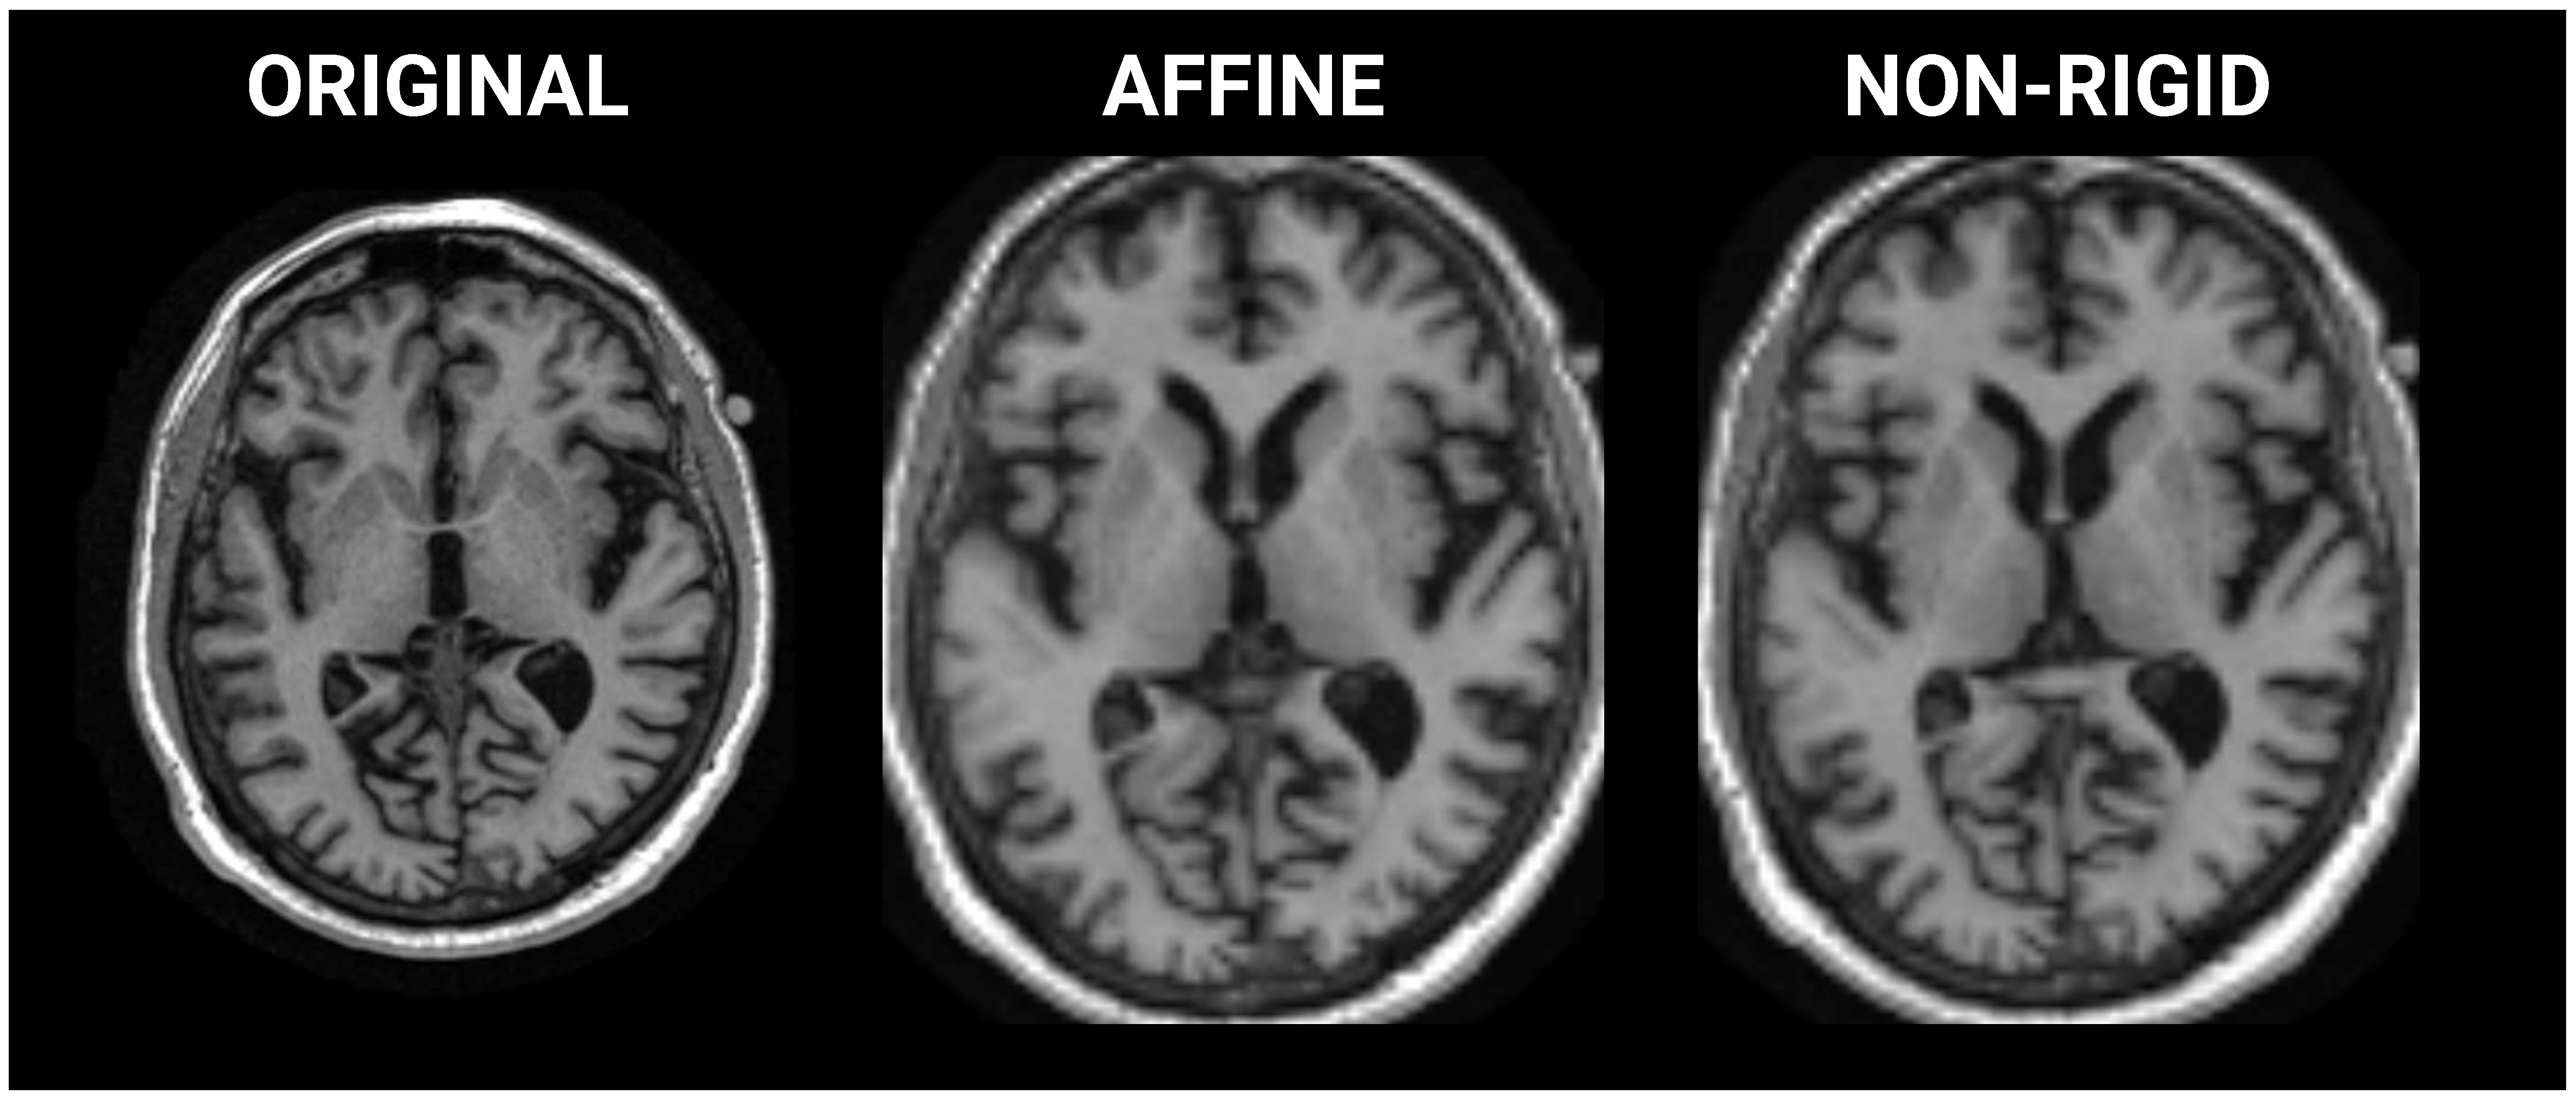
\includegraphics[width=.7\linewidth]{gfx/ch3/regComparisonMRI}}
	 \\
	\subfloat[Comparison in \ac{PET}.]
	{\includegraphics[width=.7\linewidth]{gfx/ch3/regComparisonPET}}
	\caption[Comparison of the affine registration and the application of non-linear transformations to the images]{Comparison of the affine registration and the application of non-linear transformations to the images in both \ac{MRI} and \ac{PET} modalities.}\label{fig:diffeomorphisms}
\end{figure}


\subsubsection{Co-registration}
Sometimes we have several image modalities of the same subject, for example \ac{MRI} and \ac{PET} or functional \ac{MRI}, often acquired at the same time. In this particular case, we can use the higher resolution \ac{MRI} image to calculate the affine parameters and warping, and apply those to all modalities of the same subject. To do so, we perform a first co-registration, that is, a registration of the lower-resolution images (e.g. \ac{PET}) to its correspondent \ac{MRI} image. Being anatomically similar, the co-registration usually comprises a single affine transformation. Afterwards, we can proceed with the registration of that \ac{MRI} image to the template, and apply the same transformation to all its co-registered images. 

\subsubsection{The MNI Space}
In this thesis, all images are coregistered to the \acf{MNI} space \cite{Mazziotta2001}. This is the most widely used coordinate system, recently adopted by the International Consortium for Brain Mapping (ICBM) as its standard template. The three-dimensional coordinate system defined in \ac{MNI} was intended to replace the Tailarach space, a system based on a dissected brain, that was used to compose an atlas by Tailarach and Tournoux \cite{Talairach1988c}. The current template is known as ICBM152, and features the average of 152 normal \ac{MRI} scans matched to an older \ac{MNI} template using a nine parameter affine registration. 

\subsection{Segmentation}
When using \ac{MRI} images in this thesis, we often refer to \acf{GM} and \acf{WM} maps, which is the result of the segmentation of the original data. Segmentation aims at producing maps of the distribution of different tissues, and it generally addresses \ac{GM}, \ac{WM} and \ac{CSF} classes, although lately some software can output data for bone, soft tissue or very detailed functional regions and subregions \cite{Fischl2002}. 

In this thesis we have used the \ac{VBM} toolbox of the \ac{SPM8} software, which yields \ac{GM}, \ac{WM} and \ac{CSF} maps. It features an \ac{EM} algorithm to model the distribution of the tissue classes as a mixture of gaussians and, by combining this distribution-based information with tissue probability maps using a bayesian rule, the software produces joint posterior probability maps for each tissue. To clean up the segmentation maps, a series of iterative dilations and erosions are used. Finally, since brain regions are expanded or contracted at the spatial normalization step, we can scale the segmented maps using modulation, producing final maps where the total amount of grey matter is preserved. 
%DONE

\section{Intensity Normalization}
Most functional neuroimaging modalities, in contrast to unitless structural MRI images, are the representation of the distribution of a certain contrast over the brain. There exist a larger number of sources of variability that can affect the final values: contrast uptake, radiotracer decay time, metabolism, etc.  In order to establish comparisons between subjects, an intensity normalization procedure is required. 

Intensity normalization methods are to be linear in nature, since it is essential to keep the intensity ratio between brain regions, acting on the whole brain. In its simplest form it consists of a division by a constant. This parameter is often estimated [6, 7] as the average value of the 95th bin of the histogram of the image, that is, the average of the 5\% higher intensity values, in what is known as the normalization to the maximum. Another approach, called integral normalization, estimates this parameter as the sum of all values of the image. A more complex approach requires a priori knowledge of the distribution of intensity in a normal subject. This is designed so that the whole image is divided by the Binding Potential (BP) [43], a specific-to-non-specific ratio between the intensities in areas where the tracer should be concentred and the non-specific areas. 

Then, we have general linear transformations, defined as . These procedures use estimates of the probability density function (PDF) of the source images and then estimate the parameters a and b, that transform their original PDF to an expected range. Methods to estimate the PDF parameters range from the simplest, non-parametric histogram [44] to more advanced estimates such as an ANCOVA approach used in SPM [44, 45], or parametric estimates involving the Gaussian or the more general Alpha-Stable distribution [46], which has been recently tested with great success. 

Structural modalities also suffer from some sources of intensity variability, e.g. magnetic field inhomogeneity, noise, evolution of the scanners… Field inhomogeneity causes distortions in both geometry and intensity of the MR images [47], usually addressed via increasing the strength of the gradient magnetic field or preprocessing. Intensity variability is especially noticeable in multi-centre imaging studies, where images should share certain characteristics. To improve the homogeneity of a set of structural images acquired at different locations, the use of quantitative MRI images has been recently proposed [48]. In contrast to typical unitless T1-weighted images, quantitative imaging can provide neuroimaging biomarkers for myelination, water and iron levels that are absolute measures comparable across imaging sites and time points. 
\subsection{Normalization to the Maximum}
\subsection{Integral Normalization}

\section{Voxel-wise Analyses}\label{sec:vwanalyses}
To overcome the time-consuming procedure of the traditional analysis of ROIs, several algorithms that act at the voxel level have been proposed. These include the statistical parametric mapping (SPM), a voxel-based morphometry (VBM) or the first machine learning approach in this chapter, called voxel as features (VAF). 

\subsection{Statistical Parametric Mapping}
Statistical Parametric Mapping (SPM) was proposed by Friston [45] to automatically examine differences in brain activity during functional imaging studies involving fMRI or PET. The technique can be applied to both single images (PET) and timeseries (fMRI), and the idea behind it is construct a General Linear Model (GLM) to describe the variability in the data in terms of experimental and confounding effects. 

The level of activation is assessed at a voxel level using univariate statistics, and featuring a correction for Type I errors (false positives), due to the problem of multiple comparisons. In the case of timeseries analysis, a linear convolution of the voxel signal with an estimation of the hemodynamic response is performed, and then the activation is tested against the analysed task. 

The representation of the activation is frequently presented as an overlay of the Z-scores obtained for each voxel after the multiple comparisons correction on a structural image. The Z-score –or standard score- is the signed number of standard deviations an observation is above the mean. The resulting maps allow a visual inspection of the active brain areas, which can later be related to a certain disease or task. 
\subsection{Voxel Based Morphometry}
Voxel Based Morphometry (VBM) is the application of SPM to structural MRI images [4]. The principle behind VBM is the registration to a template, and then a smoothing of the structural image so that the smaller anatomical differences between subjects are reduced. Finally, a GLM is applied voxelwise to all the images, in order to obtain a Z-score map that highlights the areas where the differences are greater. 

As commented in Section 2.2, the size of the smoothing kernel is an important parameter. A small kernel will lead to artifacts in the Z-maps, including misalignment of brain structures, differences in folding patterns or misclassification of tissue types. On the other hand, a larger kernel will not be able to detect smaller regions. 

Newer algorithms expand the idea behind VBM using multivariate approaches, to reveal different patterns. These algorithms include an Independent Component Analysis (ICA) decomposition of the dataset and conversion to Z-scores, called Source Based Morphometry (SBM) [52] and a multidimensional Tensor Based Morphometry (TBM) [53]. 

\subsection{Voxels as Features}
Voxel-As-Features (VAF) is another voxel-wise approach proposed in [5] for the diagnosis of Alzheimer’s Disease using functional imaging. It can be considered the first machine learning approach in this chapter, since it features a linear Support Vector Machine (SVM) classifier whose input features are the intensities of all voxels in the images. It has been used in many works [6, 13, 25, 32, 33] as a baseline and an estimation of the performance achieved by expert physicians by means of visual analysis. 
Additionally, some improvements can be done over the raw VAF, for example, using statistical hypothesis testing to obtain the most significant voxels, thus reducing the computational load and increasing the accuracy. The weight vector of the linear SVM can be inverse transformed to the dimension of the original images, and therefore provide a visual map that reflects the most influential voxels, in a similar way to the Z-maps of SPM and VBM. 